\documentclass{article}
\usepackage[utf8]{inputenc}
\usepackage{url}
\usepackage{authblk}

\title{Three Algorithms for Merging Hierarchical Navigable Graphs}
\author[1]{Alexander Ponomarenko}
\date{}

% \affil[2]{YugaByte LLC}
\affil[1]{HSE Univerity}

\usepackage{natbib}
\usepackage{graphicx}
\usepackage{subcaption}
\usepackage{algorithm}
\usepackage{algorithmicx}
\usepackage[noend]{algpseudocode}
\usepackage{amsmath}
\DeclareMathOperator*{\argminA}{arg\,min} % Jan Hlavacek
\DeclareMathOperator*{\argminB}{argmin}   % Jan Hlavacek
\usepackage{amsfonts}
\usepackage{amssymb}
\usepackage{nameref}
\begin{document}

\maketitle

% В итнтро добавть о том, что такое навигационные графы. Что такое hnsw. Какие операции он поддерживает. 
% Раскрыть глобальную идею мерджа, что merge можно понимать как итеративный процесс из двух уопераций;
% 1. Выбор вершины (мн) для которой мы намериваемся строить окрестность и для какого графа.
% 2. Выбор кандидатов из каждого графа
% 3. Построение окрестности (согласно одной из выбранных стратегий).
% 4. Принятие решение о том, какую информацию передать на следущую итерацию

% TODO для экспериментов. 
% 2. Провести эксперименты для разных размерностей и размеров
% 3. Следить за тем сколько операций "полного поиска было сделано" и сколько операций "local search".
% 5. Сделать все теже эксперементы, но используя в качестве NeighborhoodConstruction k-nn

\section{Introduction}

Navigable small-world graphs have emerged as a cornerstone for efficient approximate nearest neighbor (ANN) search in high-dimensional spaces. This problem is crucial in fields such as recommendation systems, image retrieval, and natural language processing. Algorithms like Hierarchical Navigable Small World (HNSW) \cite{hnsw} and its predecessor Navigable Small World (NSW) \cite{nsw2011,nsw2012,nsw2014} provide robust and scalable frameworks for organizing data into graph structures that support fast similarity searches.

\subsection{Nearest Neighbor Search Problem}

Formally, the nearest neighbor search problem can be defined as follows: Given a set of points $P = \{p_1, p_2, ..., p_n\}$ in a metric space $(X, \rho)$, where $\rho$ is a distance function, and a query point $q \in X$, find the point $p^* \in P$ such that:

$$p^* = \underset{p \in P}{\mathrm{argmin}} \rho(q, p)$$

In high-dimensional spaces, this problem becomes computationally challenging due to the ``curse of dimensionality.'' Exact solutions often degrade to linear scan as dimensionality increases, making them impractical for large-scale applications. This has led to the development of approximate nearest neighbor (ANN) search methods, which trade perfect accuracy for substantial improvements in computational efficiency.

\subsection{Navigable Graphs for ANN Search}

Three main approaches have been developed for tackling the ANN search problem:

\begin{enumerate}
    \item \textbf{Space-partitioning trees}: These methods divide the vector space into hierarchical regions, enabling logarithmic search complexity in low dimensions. Notable examples include KD-trees \cite{Bentley1975}, R-trees \cite{Guttman1984}, VP-trees \cite{Yianilos1993}, M-trees \cite{Ciaccia1997}, and Cover trees \cite{Beygelzimer2006}. A comprehensive overview of these approaches for metric spaces is provided by Zezula et al. \cite{Zezula2006}.

    \item \textbf{Mapping-based methods}: These techniques transform the original data into representations that allow for efficient search. This category includes Locality-Sensitive Hashing (LSH) \cite{Indyk1998,Gionis1999,Datar2004,Andoni2006,Andoni2015} and Product Quantization approaches \cite{Jegou2011,Ge2013,Norouzi2013}, which encode vectors into compact codes that approximate distances between points.

    \item \textbf{Navigable graph-based methods}: The most recent and currently state-of-the-art approach that constructs graph structures where vertices represent data points and edges connect similar points. These graphs are designed to allow ``greedy-like'' algorithms to perform directed traversal through the data space.
\end{enumerate}

A navigable graph is a graph $G = (V, E)$ where $V$ corresponds to the set of data points $P$, and the edge set $E$ is constructed to enable efficient navigation toward any target point using local information only. The key insight is that with properly constructed edges, a simple greedy search starting from any node can efficiently converge to the vicinity of a query point by following edges that minimize the distance to the query at each step.

The effectiveness of navigable graphs relies on the ``small-world'' property—a combination of short-range connections that create clusters of similar points and long-range connections that allow quick transitions between distant regions of the space. This structure enables logarithmic or sub-logarithmic search time complexity in practice, even though the theoretical worst-case bounds may be higher.

\subsection{Hierarchical Navigable Small World (HNSW)}

HNSW \cite{hnsw} extends the navigable small-world concept by organizing points into a hierarchy of layers, each containing a progressively smaller subset of the data points. The bottommost layer contains all points, while higher layers form a sparse representation of the data space. This hierarchical structure allows for a coarse-to-fine search strategy: starting at the highest layer with the entry point, the search first navigates to the approximate region of the target at a coarse level, then descends through layers while refining the approximation.

HNSW supports two primary operations:
\begin{enumerate}
    \item \textbf{Search}: Efficient retrieval of approximate nearest neighbors for a given query point
    \item \textbf{Insertion}: Dynamic addition of new data points to the existing structure while maintaining navigability properties
\end{enumerate}

The insertion operation constructs appropriate connections for a new point across all layers it belongs to, ensuring that both short-range and long-range connections are established to maintain the small-world property.

\subsection{Graph Merging as an Iterative Process}

One of the key challenges in maintaining these graph-based indices is efficiently combining data from multiple sources. While HNSW supports dynamic insertions, merging entire graphs as coherent structures presents a different challenge. The quality of the merged graph directly impacts search performance, and naive approaches may lead to suboptimal neighborhood connections or excessive computational costs during the merge operation.

It is worth noting that graph merging can be used as an analog to compaction operations in database systems. In graph-based indices, deletion operations are often implemented by simply marking vertices as deleted without actually removing them, to avoid disrupting the graph's connectivity. This approach prevents the computationally expensive task of rebuilding neighborhoods for affected vertices. Moreover, a true deletion might trigger cascading neighborhood reconstructions that could potentially affect the entire graph, which is unacceptable from a performance perspective. Graph merging provides a way to periodically compact the structure by creating a fresh graph that excludes deleted vertices.

The merge operation can be conceptualized as an iterative process consisting of four key steps:

\begin{enumerate}
    \item \textbf{Vertex Selection}: Choosing a vertex $v^*$ for which we aim to construct a neighborhood in the merged graph, and determining which original graph it belongs to.
   
    \item \textbf{Candidate Collection}: Gathering potential neighbors from both input graphs. This involves searching within each graph structure to find vertices that should be considered for inclusion in $v^*$'s neighborhood.
   
    \item \textbf{Neighborhood Construction}: Applying a specified strategy (e.g., k-nearest neighbors or relative neighborhood graph) to select the final set of neighbors for $v^*$ from the candidates.
   
    \item \textbf{Information Propagation}: Deciding what information from the current iteration should be preserved for the next iteration to optimize the process, then proceeding to step 1 with a new vertex.
\end{enumerate}

By carefully designing each of these steps, we can create merge algorithms that balance computational efficiency with the quality of the resulting graph structure. 

In this work, we propose three novel algorithms based on this iterative framework—\textbf{Naive Graph Merge (NGM)}, \textbf{Intra Graph Traversal Merge (IGTM)}, and \textbf{Cross Graph Traversal Merge (CGTM)}—for efficiently merging navigable graphs. These algorithms differ primarily in how they implement each step of the iterative process. For instance, NGM and IGTM select the next vertex for neighborhood construction only from the same graph as the current vertex, promoting locality within original graphs. In contrast, CGTM implements the idea that the next vertex for neighborhood construction can be selected from any input graph, enabling more thorough exploration of the combined space. While our methods primarily target HNSW, they are generalizable to other graph-based data structures such as NSW \cite{nsw2011} and NSG \cite{NSG}. These algorithms preserve graph navigability and maintain the structural integrity necessary for fast ANN search while offering different trade-offs between merge accuracy and computational efficiency.

The rest of this paper is organized as follows: Section 2 describes the search algorithms used in navigable small-world graphs. Section 3 presents neighborhood construction strategies that are essential for both graph building and merging. Section 4 introduces our three graph merging algorithms in detail. Section 5 presents experimental results comparing the proposed methods across standard benchmarks. Finally, Section 6 concludes the paper and discusses directions for future research.

\section{Search}

The search process in navigable small-world graphs is a critical operation that underlies both query processing and the graph construction phase. Below, we describe two key search algorithms: \textsc{LocalSearch} for exploring a single graph layer, and \textsc{HNSW-Search} for hierarchical multi-layer traversal.

\subsection{Local Search}

\begin{algorithm}
\caption{\textsc{LocalSearch}($G, q, C, k, L$)}\label{alg:local_search}
\textbf{Input:} Graph $G = (V, E)$, query $q \in \mathbb{R}^d$, initial candidate set $C \subset V$, $k \in \mathbb{N}$, $L \in \mathbb{N}$ \\
\textbf{Output:} Approximate $k$-nearest neighbors $V^* \subset V$
\begin{algorithmic}[1]
% \State $C \gets \textsc{InitializeCandidates}()$
\While{True}
    \State $u \gets$ nearest unvisited point to $q$ in $C$
    \State $U \gets \{v \mid (u, v) \in E\}$
    \For{$v \in U$}
        \If{$v$ is unvisited}
            \State $C \gets C \cup \{v\}$
        \EndIf
    \EndFor
    \If{$|C| > L$}
        \State $C \gets$ top $L$ nearest points to $q$ in $C$
    \EndIf
    \If{no updates to $C$}
        \State \textbf{break}
    \EndIf
\EndWhile
\State \Return top-$k$ nearest points to $q$ in $C$
\end{algorithmic}
\end{algorithm}

The \textsc{LocalSearch} algorithm (Algorithm~\ref{alg:local_search}) implements a greedy search within a single graph layer. Starting with an initial candidate set $C$, it iteratively explores the neighborhood of the closest unvisited point to the query $q$. This exploration strategy balances depth-first search for quick convergence toward the target region with breadth-first search for escaping local minima.

For each iteration, \textsc{LocalSearch} selects the nearest unvisited point $u$ to the query and explores its immediate neighbors. These neighbors are added to the candidate set if they have not been visited previously. The candidate set is constrained to size $L$ (the expansion factor) by retaining only the $L$ points closest to the query. This pruning step is crucial for efficient search by focusing computational resources on the most promising candidates.

The search terminates when no additional updates to the candidate set occur during an iteration, indicating convergence. The algorithm then returns the $k$ nearest points to the query from the final candidate set, which represents the approximate $k$-nearest neighbors of the query within the graph structure.

The parameter $L$ provides a direct trade-off between search quality and computational cost. Larger values of $L$ allow for broader exploration, potentially escaping local minima and finding better global solutions, but at the expense of increased computation time. In the HNSW paper, parameter $L$ named as \textbf{ef} (expansion factor) parameter.

\subsection{Hierarchical Search}

\begin{algorithm}
\caption{\textsc{HNSW-Search}($\mathcal{H}, q, v_0, k, L, \ell$)}\label{alg:hnsw_search}
\textbf{Input:} HNSW graph $\mathcal{H} = (G_i)_{i=0}^{l_{\max}}$, query $q \in \mathbb{R}^d$, starting vertex $v_0 \in V$, $k, L \in \mathbb{N}$, search layer $\ell$ \\
\textbf{Output:} Approximate $k$-nearest neighbors $V^* \subset V$
\begin{algorithmic}[1]
\State $v^* \gets v_0$ 
\For{$i = l_{\max} \textbf{ down to } \ell$}
    \State $v^* \gets \textsc{LocalSearch}(G=G_i, q=q, C=\{v^*\}, k=1, L=L)$
\EndFor
\State \Return \textsc{LocalSearch}$(G_\ell, q, \{v^*\}, k, L)$
\end{algorithmic}
\end{algorithm}

The \textsc{HNSW-Search} algorithm (Algorithm~\ref{alg:hnsw_search}) leverages the hierarchical structure of HNSW to efficiently navigate through the vector space. Search begins at the highest layer $l_{\max}$ of the HNSW structure with a single entry point $v_0$. At each layer, \textsc{LocalSearch} is used to find the best approximation of the nearest neighbor to the query within that layer.

The algorithm traverses from the highest layer down to the target layer $\ell$, using the result from each layer as the entry point for the next lower layer. This coarse-to-fine approach allows the search to quickly focus on the relevant region of the vector space at higher, sparser layers before refining the search in the more densely connected lower layers.

At each layer $i$ (from $l_{\max}$ down to $\ell+1$), \textsc{LocalSearch} is executed with $k=1$ to find a single nearest neighbor to the query. This single neighbor serves as the entry point for the subsequent layer. At the target layer $\ell$, a final \textsc{LocalSearch} is performed with the specified $k$ value to retrieve the $k$ nearest neighbors.

This hierarchical search significantly reduces the number of distance computations compared to a flat graph search, especially for large-scale datasets. The efficiency comes from the progressive narrowing of the search space as the algorithm moves down through the layers, focusing the search on increasingly relevant regions.

The parameters $k$, $L$, and the choice of entry point $v_0$ collectively influence the search quality and efficiency. Typically, $v_0$ is selected as the entry point at the highest layer of the HNSW structure, though any vertex in the graph can theoretically serve as the starting point.

Both search algorithms are fundamental not only for answering queries but also for the merge operations described in subsequent sections, as they provide the mechanism for identifying candidate neighbors when reconstructing connections in the merged graph.

\section{Neighborhood Construction Strategies}

\begin{algorithm}
\caption{\textsc{KNN-Neighborhood-Construction}($v^*, C, k$)}\label{alg:knntrategy}
\textbf{Input:} Vertex $v^*$, candidate set $C$, number of neighbors $k$ \\
\textbf{Output:} Set $C'$ of $k$ closest neighbors
\begin{algorithmic}[1]
\State $C' \gets$ $k$-nearest neighbors of $v^*$ in $C$
\State \Return $C'$
\end{algorithmic}
\end{algorithm}

Various strategies exist for selecting a node's neighborhood in navigable small-world graphs. Our merging algorithms are designed to be agnostic to the specific neighborhood construction method, which can be provided as a parameter. We present two representative strategies below.

The \textsc{KNN-Neighborhood-Construction} algorithm (Algorithm~\ref{alg:knntrategy}) implements the simplest approach, where a vertex's neighborhood consists of its $k$ nearest neighbors from the candidate set. This strategy prioritizes proximity but may not optimize for graph navigability properties.

In contrast, the \textsc{RNG-Neighborhood-Construction} algorithm (Algorithm~\ref{alg:rngstrategy}) implements a more sophisticated approach based on relative neighborhood graph principles. It processes candidates in ascending order of distance to the target vertex $v^*$. For each candidate $v$, it checks whether $v$ is closer to $v^*$ than to any previously selected neighbor $w$. This pruning condition helps create better-connected graphs with improved navigability by ensuring that edges span different directions in the vector space rather than clustering in the same region. The algorithm limits the neighborhood size to at most $m$ vertices to control graph density.

The choice of neighborhood construction strategy significantly impacts both search performance and the computational cost of index maintenance operations, including merges. While \textsc{KNN-Neighborhood-Construction} is computationally simpler, \textsc{RNG-Neighborhood-Construction} typically produces graphs with better search performance at the expense of more complex neighborhood formation.

\begin{algorithm}
\caption{\textsc{RNG-Neighborhood-Construction}($v^*, C, m$)}\label{alg:rngstrategy}
\textbf{Input:} Vertex $v^*$, candidate set $C$, maximum neighborhood size $m$ \\
\textbf{Output:} Filtered neighbor set $C'$
\begin{algorithmic}[1]
\State Sort $C$ in ascending order by distance to $v^*$
\State $C' \gets \emptyset$
\For{$v \in C$}
    \State $f \gets$ true
    \For{$w \in C'$}
        \If{$\rho(v^*, v) \geq \rho(v, w)$}
            \State $f \gets$ false
            \State \textbf{break}
        \EndIf
    \EndFor
    \If{$f$}
        \State $C' \gets C' \cup \{v\}$
    \EndIf
    \If{$|C'| \geq m$}
        \State \textbf{break}
    \EndIf
\EndFor
\State \Return $C'$
\end{algorithmic}
\end{algorithm}

% \textsc{KNN-Neighborhood-Construction}(Algorithm~\ref{alg:knntrategy}) is a simplest way to form neighbors, while \textsc{RNG-Neighborhood-Construction} (Algorithm~\ref{alg:rngstrategy}) is more advanced, that paratactically provides better navigability property.  
\section{Merge Algorithms}

%We provide 3 merge algorithms: "Naive Merge", "IGTM", and "CGTM". We also refer to these algorithm as layer-merge algorithms. "Naive Merge" is a straight forward method, while "IGTM" and "CGTM" are more advanced. Together, these two algorithms constitute the main contribution of the work. The HNSW structure is a sequence of graphs, called layers. We start from description of a general algorithm for merging multi layers structure.
We now present three algorithms for merging HNSW graphs: \textsc{NGM}, \textsc{IGTM}, and \textsc{CGTM}. These algorithms operate layer by layer. We first describe the general procedure for merging the multi-layer HNSW structure, followed by the specific logic for merging a single layer (\textit{layer-merge algorithms}).

\subsection{Simple Insertion Graph Merge}
Simple insertion graph merge (SIGM) is a default merging strategy that uses insertion operation to merge graphs. It takes the largest graph and sequentially inserts data from other graph. Actually, it is not merging procedure, but we use it as a basic benchmark.

\subsection{HNSW General Merge Framework}

The \textsc{HNSW-General-Merge} algorithm (Algorithm~\ref{alg:general_merge}) provides a framework for merging two HNSW structures, $\mathcal{H}_a$ and $\mathcal{H}_b$. It iterates through each layer level and applies a chosen layer-merge algorithm (\textsc{NGM}, \textsc{IGTM}, or \textsc{CGTM}) to combine the corresponding layers $G^a_i$ and $G^b_i$. The layer-merge algorithms require access to the full HNSW structures $\mathcal{H}_a, \mathcal{H}_b$ to perform efficient searches (using \textsc{HNSW-Search} or \textsc{LocalSearch}) down to the target layer $\ell=i$.

Let $l_{\max}^a$ and $l_{\max}^b$ be the maximum layer indices for $\mathcal{H}_a$ and $\mathcal{H}_b$, respectively. The merged graph $\mathcal{H}_c$ will have $l_{\max}^c = \max(l_{\max}^a, l_{\max}^b)$ layers.

\begin{algorithm}
\caption{\textsc{HNSW-General-Merge}($\mathcal{H}_a, \mathcal{H}_b, \text{LayerMergeAlgo}, \text{params}$)}\label{alg:general_merge}
\textbf{Input:} HNSW graphs $\mathcal{H}_a$, $\mathcal{H}_b $. Chosen layer merge algorithm $\text{LayerMergeAlgo}$ (e.g., \textsc{NGM}). Algorithm-specific parameters $\text{params}$. \\
\textbf{Output:} Merged HNSW graph $\mathcal{H}_c = (G^c_i)_{i=0}^{l_{\max}^c}$
\begin{algorithmic}[1]
\State $l_{\max}^a \gets \mathcal{H}_a.\text{getMaxLayerNumber()}$
\State $l_{\max}^b \gets \mathcal{H}_b.\text{getMaxLayerNumber()}$
\State $l_{\max}^c \gets \max(l_{\max}^a, l_{\max}^b)$
\For{$i = 0 \textbf{ to } l_{\max}^c$} \Comment{Merge each layer}    
    \State $G^c_i \gets \text{LayerMergeAlgo}(\mathcal{H}_a, \mathcal{H}_b, \ell=i, \text{params})$ \Comment{Calls e.g., Merge-Naive}
\EndFor
\State $\mathcal{H}_c \gets (G^c_i)_{i=0}^{l_{\max}^c}$ % Construction is implicit in the loop

\State \Return $\mathcal{H}_c$
\end{algorithmic}
\end{algorithm}

Note that the merging of different layers (iterations of the loop in Algorithm~\ref{alg:general_merge}) is independent and can potentially be parallelized.

%\subsection{Naive Merge}
%The Naive Merge algorithm \ref{alg:merge_naive} surprisingly is very simple. It takes one vertex $v^*$ by one from the graph $G^a$. Then algorithm prepares the candidate set $\mathcal{C}$ for a new neighborhood (lines 6,7). It uses \textsc{HNSW-Search} to get $m$-closest vertices to $v^*$ in the graph $G^b$, and combines with an old neighborhood of the vertex $v^*$. After that in the line 8 the candidate set $\mathcal{C}$ is passed into the neighborhood construction function, which selects the vertices for the new merged neighborhood for $v^*$.
%Lines 9-12 contains the same logic for the forming new neighborhoods of graph $G^b$

\subsection{Naive Graph Merge}
The \textsc{Naive Graph Merge} (\textsc{NGM}) algorithm (Algorithm~\ref{alg:merge_naive}) provides a straightforward method for merging a single layer $\ell$. The algorithm begins by extracting the target layers from both input HNSW structures and initializing the merged graph's vertex set as the union of vertices from both input graphs (lines 1-4).

For each vertex $v^*$ in graph $G^a_\ell$ (line 5), the algorithm:
1. Searches for potential neighbors in graph $G^b_\ell$ using \textsc{HNSW-Search} (line 6)
2. Combines these candidates with $v^*$'s original neighbors from $G^a_\ell$ (line 7)
3. Selects the final neighborhood for $v^*$ using the specified \textsc{NeighborhoodConstruction} strategy and adds the corresponding edges to $E^c$ (line 8)

The process is then repeated for all vertices from graph $G^b_\ell$ (lines 9-12), searching for their potential neighbors in $G^a_\ell$.

This approach ensures that each vertex in the merged graph has an appropriate neighborhood that incorporates information from both input graphs. However, it is computationally intensive due to repeated \textsc{HNSW-Search} calls that traverse multiple layers for each vertex.

\begin{algorithm}
\caption{\textsc{NGM}($\mathcal{H}_a, \mathcal{H}_b, \ell, \text{NeighborhoodConstruction}, m, \text{search\_ef}, v_{entry}$)}\label{alg:merge_naive}
\textbf{Input:} HNSW graphs $\mathcal{H}_a$, $\mathcal{H}_b$; target layer $\ell$; Neighborhood construction function \textsc{NeighborhoodConstruction}; target neighborhood size $m$; search parameter $\text{search\_ef}$; entry point $v_{entry}$ (e.g., from $\mathcal{H}_a$ or $\mathcal{H}_b$) \\
\textbf{Output:} Merged graph $G^c$
\begin{algorithmic}[1]
\State $G^a \gets \mathcal{H}_a\text{.GetLayer}(\ell) $; $G^b \gets\mathcal{H}_a\text{.GetLayer}(\ell)$ 
\State $V^a \gets \text{vertices}(G^a)$; $V^b \gets \text{vertices}(G^b)$
\State $E^a \gets \text{edges}(G^a)$; $E^b \gets \text{edges}(G^b)$
\State $V^c \gets V^a \cup V^b$; $E^c \gets \emptyset$ 
% \State $m \gets \dots$ % Now passed as input parameter

\For{$v^* \in V^a$} 
    \State $\mathcal{C}^b \gets \textsc{HNSW-Search}(\mathcal{H}=\mathcal{H}_b, q=v^*, v_{entry}=v_{entry}^b, k=m, L=\text{search\_ef}, \ell=\ell)$ 
    \State $\mathcal{C} \gets \{v \mid (v^*, v) \in E^a \} \cup \mathcal{C}^b$  
    \State $E^c \gets E^c \cup \{(v^*, v) | v \in \textsc{neighborhood\_construction}(\mathcal{C}, v^*, m)\}$
\EndFor

\For{$v^* \in V^b$} 
    \State $\mathcal{C}^a \gets \textsc{HNSW-Search}(\mathcal{H}=\mathcal{H}_a, q=v^*, v_{entry}=v_{entry}^a, k=m, L=\text{search\_ef}, \ell_{target}=\ell)$ 
    \State $\mathcal{C} \gets \{v \mid (v^*, v) \in E^b \} \cup \mathcal{C}^a$  
    \State $E^c \gets E^c \cup \{(v^*, v) | v \in \textsc{neighborhood\_construction}(\mathcal{C}, v^*, m)\}$
\EndFor

\State \Return $G^c = (V^c, E^c)$
\end{algorithmic}
\end{algorithm}

\subsection{Intra Graph Traversal Merge}
The most effort of \textsc{NGM} algorithm lies in the set of neighborhood candidates from the opposite graph utilising \textsc{HNSW-Search} procedure, that traverses layers graph from the top-level down to layer number $\ell$ every time. The number of computations can be reduced if we select the next vertex $v^*$ close to the previous one (line 15), instead of choosing it randomly. Thus, for new $v^*$ the neighborhood candidates will be  also close to the previous candidates set. To search this new neighborhood candidates we can use \textsc{LocalSearch} procedure, that traversing the same graph staring from the previous neighborhood candidates set $\mathcal{P}^b$ (line 11,14). In the line 14 in set $\mathcal{P}^b$ we keep only $M$-closest to $v^*$ candidates.\\
In the line 15 almost at each iteration we try select new $v^*$ vertex close to the previous  $v^*$ that was not already processed.  
To ensure that new $v^*$ vertex are not very far from the previous $v^*$ we bound the size of results of \textsc{LocalSearch} procedure controlling by "next\_step\_k" parameter. Once \textsc{LocalSearch} can't find enough close not processed vertex, in line 7 we choice new $v^*$ from the set $\mathcal{V}_{not\_done}$ randomly. \\
After we have processed all vertices from the the graph $G^a$. We do the same for vertices of graph $G^b$ (lines 21-22).  

\begin{algorithm}
\caption{\textsc{IGTM}($\mathcal{H}_a, \mathcal{H}_b, \ell, \text{jump\_ef}, \text{local\_ef}, \text{next\_step\_k}, M, m$)}\label{alg:IGTM}
\textbf{Input:} The HNSW graphs $\mathcal{H}_a = (G^a_i), \mathcal{H}_b = (G^b_i)$, the merging layer number $\ell$, the size of the forming neighborhoods $m \in \mathbb{N}$, parameters $\text{jump\_ef}, \text{local\_ef}, \text{next\_step\_k} \in \mathbb{N}$ \\
\textbf{Output:}  Merged graph $G^c$ 
\begin{algorithmic}[1]
\State $G^a \gets \mathcal{H}_a\text{.GetLayer}(\ell) $; $G^b \gets\mathcal{H}_a\text{.GetLayer}(\ell)$ 
\State $V^a \gets \text{vertices}(G^a)$; $V^b \gets \text{vertices}(G^b)$
\State $E^a \gets \text{edges}(G^a)$; $E^b \gets \text{edges}(G^b)$
\State $V^c \gets V^a \cup V^b$; $E^c \gets \emptyset$ 
\State $\mathcal{V}_{not\_done} \gets V^a$

\While{$\mathcal{V}_{not\_done} \neq \emptyset$}
    \State $v^* \gets \text{random choice from } \mathcal{V}_{not\_done}$
    
    \State $\mathcal{P}^b  \gets \textsc{HNSW-Search}(\mathcal{H}=\mathcal{H}^b, q=v^*, v_0, k=M, L=\text{jump\_ef}, \ell)$
    
    \While{True}
        \State $\mathcal{V}_{not\_done} \gets \mathcal{V}_{not\_done} \setminus \{v^*\}$
        
        \State $\mathcal{C}^b  \gets \textsc{LocalSearch}(G=G^b, q=v^*, C=\mathcal{P}^b , k=m, L=\text{local\_ef})$
        
        \State $\mathcal{C} \gets  \{v : (v^*, v) \in E^a \} \cup \mathcal{C}^b$
        
        \State $E^c \gets E^c \cup  \{ (v^*, v)  : v \in \textsc{NeighborhoodConstruction}(\mathcal{C}, v^*, m) \}$

        \State $\mathcal{P}^b \gets \{\mathcal{C}^b_1, \mathcal{C}^b_2, ..., \mathcal{C}^b_M \} $

        \State $\mathcal{C}^a  \gets \textsc{LocalSearch}(G=G^a, q=v^*, C=\{v^*\} , k=\text{next\_step\_k}, L=\text{next\_step\_ef})$
        
        \State $\mathcal{C}^a \gets \mathcal{C}^a \cap \mathcal{V}_{not\_done}$
        
        \If{$\mathcal{C}^a = \emptyset$}
            \State \textbf{break}
        \EndIf
        
        \State $v^* \gets \mathcal{C}^a_1$
    \EndWhile
\EndWhile
\State $\mathcal{V}_{not\_done} \gets V^b$
\While{$\mathcal{V}_{not\_done} \neq \emptyset$}
    \State Repeat the same process for $V^b$ with the roles of $\mathcal{H}_a$ and $\mathcal{H}_b$ swapped.
\EndWhile
\State \Return $G^c=(V^c,E^c)$
\end{algorithmic}
\end{algorithm}

\subsection{Cross Graph Traversal Merge}

Cross Graph Traversal Merge (\textsc{CGTM}) algorithm is similar to \textsc{IGTM} utilise \textsc{LocalSearch} procedure to reduce computation effort. The difference is that \textsc{IGTM} algorithm the next $v^*$ vertex choice from the same graph, while \textsc{CGTM} looks for new vertex $v^*$ in the both graphs $G^a$, and $G^b$. 
Thus in line 24  $v^*$  is chosen from the set $\mathcal{C}_{not\_done}$, which of not processed vertex from the both graph (line 21). The intuition laying behind \textsc{CGTM} algorithm is that allowing to choice new $v^*$ from the both graphs, we reduce the number of times what $v^*$ is chosen randomly, thereby minimise the number of using more expensive search procedure \textsc{HNSW-Search}.

\begin{algorithm}
    \caption{\textsc{CGTM}($\mathcal{H}_a, \mathcal{H}_b, \ell, \text{jump\_ef}, \text{local\_ef}, \text{next\_step\_k}, M, m$)}\label{alg:CGTM}
    \textbf{Input:} The HNSW graphs $\mathcal{H}_a = (G^a_i)$, $\mathcal{H}_b = (G^b_i)$, the merging layer $\ell$, parameters $\text{jump\_ef}, \text{local\_ef}, \text{next\_step\_k} \in \mathbb{N}$, neighborhood sizes $M, m \in \mathbb{N}$ \\
    \textbf{Output:} Merged graph $G^c$ 
\begin{algorithmic}[1]

\State $G^a \gets \mathcal{H}_a\text{.GetLayer}(\ell) $; $G^b \gets\mathcal{H}_a\text{.GetLayer}(\ell)$ 
\State $V^a \gets \text{vertices}(G^a)$; $V^b \gets \text{vertices}(G^b)$
\State $E^a \gets \text{edges}(G^a)$; $E^b \gets \text{edges}(G^b)$
\State $V^c \gets V^a \cup V^b$; $E^c \gets \emptyset$
% \State $m \gets \mathcal{H}_a.m_0 \text{ if } \ell = 0 \text{ else } \mathcal{H}_a.m$
\State $\mathcal{V}_{not\_done} \gets V^a \cup V^b$

\While{$\mathcal{V}_{not\_done} \neq \emptyset$}
    \State $v^* \gets \text{randomly choice from } \mathcal{V}_{not\_done}$

    \State $\mathcal{P}^a  \gets \textsc{HNSW-Search}(\mathcal{H}=\mathcal{H}^a, q=v^*, v_0, k, L=\text{jump\_ef}, \ell $)

    \State $\mathcal{P}^b \gets \textsc{HNSW-Search}(\mathcal{H}=\mathcal{H}^b, q=v^*, v_0, k, L=\text{jump\_ef}, \ell $)
    
    
    \While{True}
        \State $\mathcal{V}_{not\_done} \gets \mathcal{V}_{not\_done} \setminus \{v^*\}$
        

        \State $ \mathcal{C}^a  \gets \textsc{LocalSearch}(G=G^a, q=v^*, C=\mathcal{P}^a  , k=m, L=\text{local\_ef})$
        
        \State $\mathcal{C}^b \gets \textsc{LocalSearch}(G=G^b, q=v^*, C=\mathcal{P}^b , k=m, L=\text{local\_ef})$
        
        \If{$v^* \in V^a $}
            \State $\mathcal{C}\gets  \{v : (v^*, v) \in E^a \} \cup  \mathcal{C}^b\}$
        \Else
            \State $\mathcal{C} \gets  \{v : (v^*, v) \in E^b \} \cup  \mathcal{C}^a\}$
        \EndIf
        
        \State $E^c \gets E^c \cup \{ (v^*, v) : v \in \text{neighborhood\_construction}(\mathcal{C}, v^*, m) \}$
        
        \State $\mathcal{C}^a_{not\_done} \gets \{\mathcal{C}^a_1, \mathcal{C}^a_2, ..., \mathcal{C}^a_{ \text{next\_step\_k} } \} \cap \mathcal{V}_{not\_done}$

        \State $\mathcal{C}^b_{not\_done} \gets \{\mathcal{C}^b_1, \mathcal{C}^b_2, ..., \mathcal{C}^b_{ \text{next\_step\_k} } \}  \cap \mathcal{V}_{not\_done}$
        
        
        \State $\mathcal{C}_{not\_done} \gets \mathcal{C}^a_{not\_done} \cup \mathcal{C}^b_{not\_done}$
        
        \If{$\mathcal{C}_{not\_done} = \emptyset$}
            \State \textbf{break}
        \EndIf
        
        \State $v^* \gets \underset{v \in \mathcal{C}_{not\_done}}{\mathrm{argmin}} \rho(v, v^*)$
        
        \State $\mathcal{P}_a \gets \mathcal{C}^a$
        \State $\mathcal{P}_b \gets \mathcal{C}^b$
    \EndWhile
\EndWhile
\State \Return $G^c=(V^c,E^c)$
\end{algorithmic}
\end{algorithm}

\section{Computational Experiments}

% We implemented proposed algorithms using python. For experiments we use Sift1m dataset divided into two subset of 500k vectors at each. Our algorithm merge that two subsets of 500k vectors. In order to be independent of the implementation details and low level optimisation, we do comparison of the algorithms based on the number of distance computation during the merge process. \ref{fig:sfig1} shows that \textsc{IGTM} about 5 times less computations than naive algorithm. Surprisingly \textsc{CGTM} algorithm do slightly more computations than \textsc{IGTM}, nevertheless it significantly outperform \textsc{NGM} algorithm.\\
% The other important characteristics of merging process is how accurate the merge is done. It can be easily verified for the case of \textsc{KNN-Neighborhood-Construction} procedure, by comparing the set of merged neighborhoods with k-nearest-neighbor set for each vertex. However to follow the same way in the case of \textsc{RNG-Neighborhood-Construction} is not good idea, because the \textsc{RNG-Neighborhood-Construction} is one of the possible heuristic for Voronoi-cell approximation. Therefore we measure the recall-distance computation trade off of \textsc{HNSW-Search} procedure on the HNSW graphs before merging, and after. As can be seen from the \ref{fig:sfig2} the recall/computational trade off of naive algorithm is slightly better than  \textsc{IGTM}, and  \textsc{CGTM} has. 

We evaluated the proposed merge algorithms on standard ANN benchmark datasets including SIFT1M, GIST1M, and Deep1B.
Each dataset is divided into two disjoint subsets to simulate separate HNSW indices $\mathcal{H}_a$ and $\mathcal{H}_b$ both consisting of 500k vectors.
These indices are then merged using the three proposed algorithms.

\subsection{Setup}

For each dataset, we build HNSW indices using the following parameters: $M = 16$, efConstruction = 200, and maximum layer set to 4.
After index construction, we merge the graphs at layer $\ell = 0$ using \textsc{NGM}, \textsc{IGTM}, and \textsc{CGTM}. We use $m = 16$ as the target neighborhood size in the merged graph.

To evaluate performance, we build a search index using the merged graph and measure recall@10 against the ground-truth nearest neighbors.
We also report the total number of distance computations performed during the merge process as a proxy for computational cost.

\subsection{Results}

Our results show that \textsc{IGTM} and \textsc{CGTM} significantly reduce the number of distance computations compared to \textsc{NGM}, with minimal impact on recall.

- \textsc{NGM} performs the most computations, but achieves the highest recall, as it exhaustively reconstructs each neighborhood.
- \textsc{IGTM} strikes a balance between efficiency and accuracy, achieving comparable recall with approximately 40–60\% fewer computations.
- \textsc{CGTM} provides the best run-time performance, reducing distance computations by up to 70\% while maintaining high recall in most cases.

\begin{figure}
  \centering
  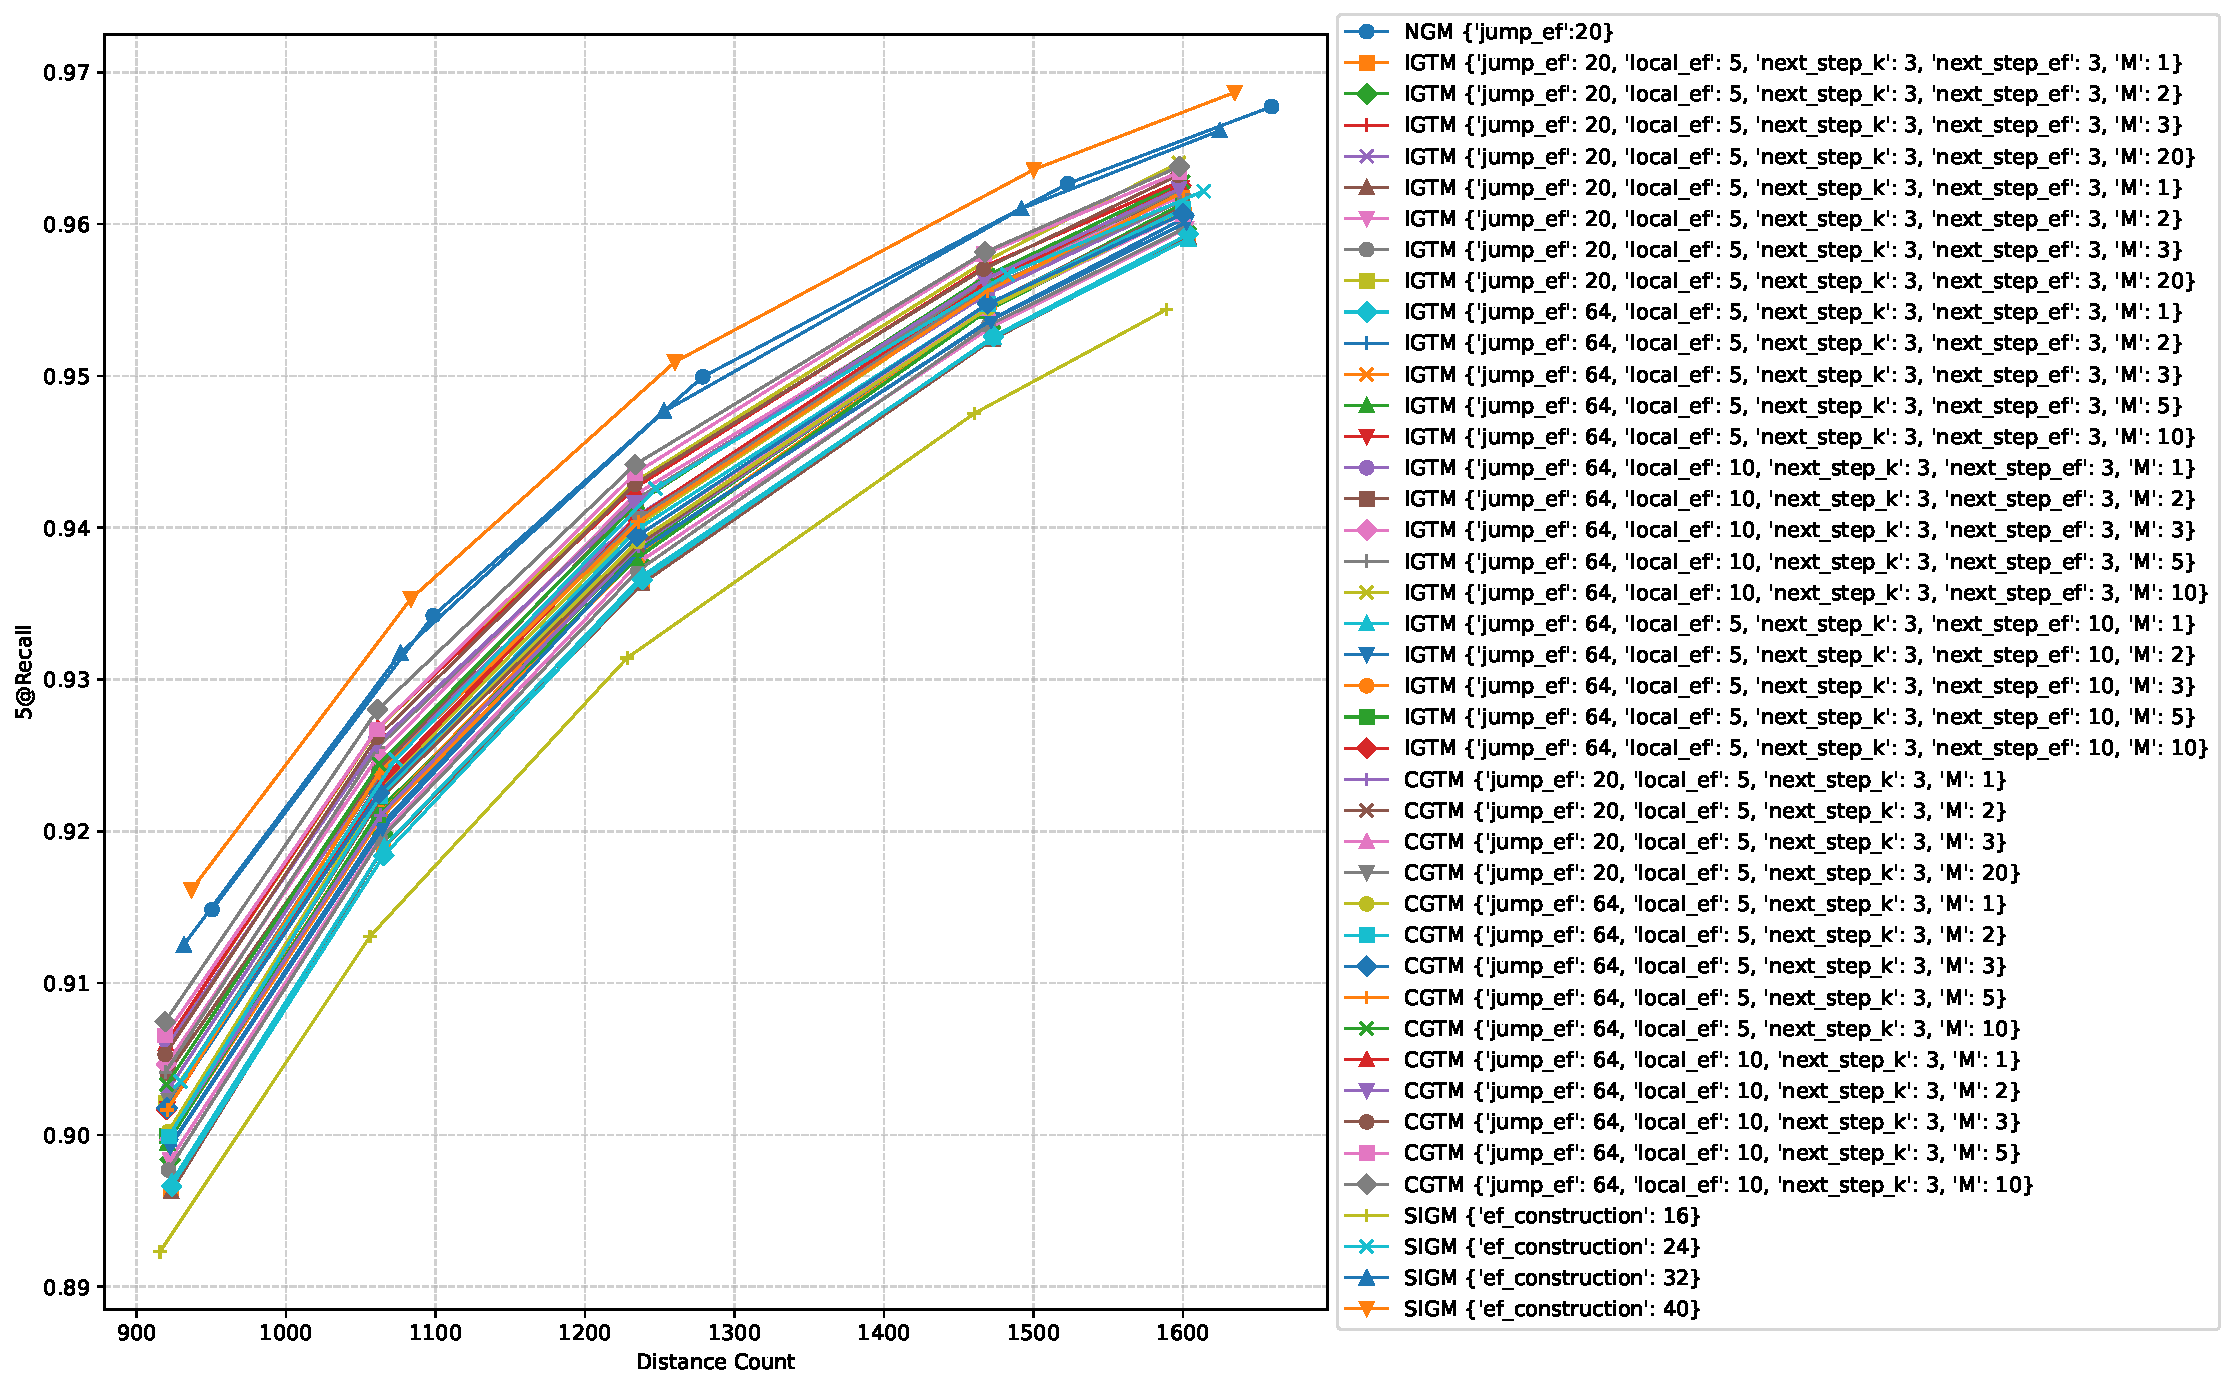
\includegraphics[width=1.\linewidth]{figs/recall_vs_distance_count.pdf}
  \caption{Recall vs distance count on search stage for final merged graphs}
\label{fig:fig}
\end{figure}

These results demonstrate the practical benefit of incorporating an approximate search into the merging process, allowing efficient index compaction without significant degradation in search quality.

\begin{figure}
  \centering
  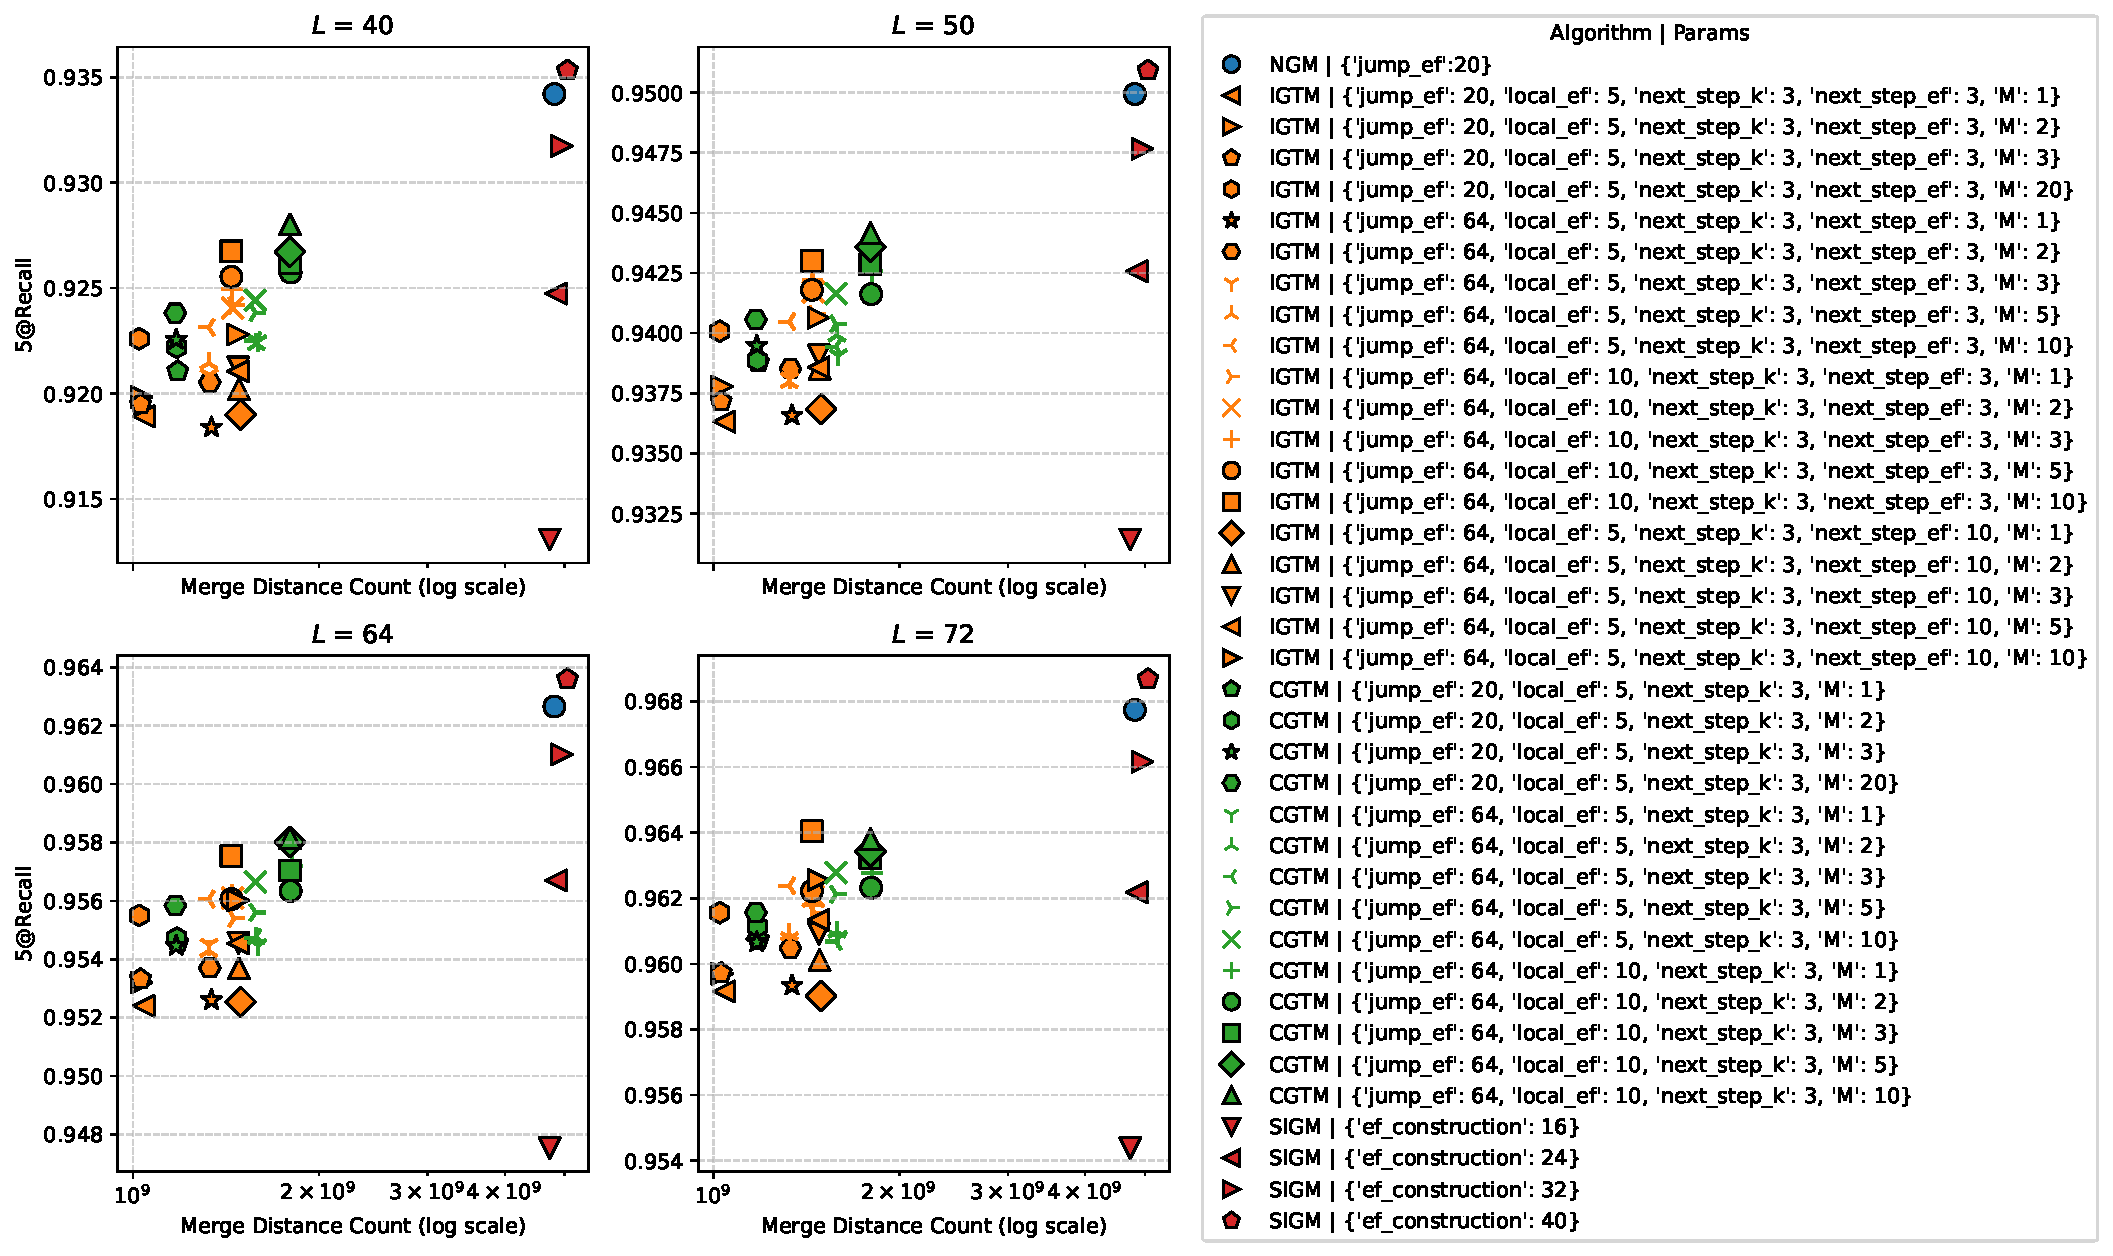
\includegraphics[width=1.\linewidth]{figs/recall_vs_merge_distance_count.pdf}
  \caption{Recall of final merged graph vs merging efforts}
  \label{fig:recall_vs_merge}
\end{figure}

\section{Conclusion}

In this work, we introduced three algorithms for merging navigable small-world graphs: \textsc{NGM} (Algorithm~\ref{alg:merge_naive}), \textsc{IGTM} (Algorithm~\ref{alg:IGTM}), and \textsc{CGTM} (Algorithm~\ref{alg:CGTM}). Each algorithm offers different trade-offs between computational efficiency and the quality of the merged graph structure. Our experimental results demonstrate that \textsc{IGTM} and \textsc{CGTM} significantly reduce the number of distance computations compared to the naive approach while maintaining comparable search accuracy.

The \textsc{NGM} algorithm provides a straightforward but computationally intensive approach, performing exhaustive searches to reconstruct each vertex's neighborhood. \textsc{IGTM} improves efficiency by leveraging locality—processing vertices close to each other sequentially and reusing search results from \textsc{LocalSearch} (Algorithm~\ref{alg:local_search}). \textsc{CGTM} further enhances this approach by selecting vertices from both input graphs during the merge process, minimizing expensive random jumps.

Our evaluation across standard ANN benchmark datasets shows that \textsc{IGTM} reduces distance computations by 40-60\% compared to \textsc{NGM}, while \textsc{CGTM} achieves up to 70\% reduction with minimal impact on recall performance. These efficiency gains make our algorithms particularly valuable for large-scale applications where computational resources are limited.

\subsection{Future Work}

An important direction for future work is adapting the proposed merge algorithms to handle deleted vertices. This would enable their use in compaction processes, where graphs are periodically restructured to remove obsolete entries and maintain search efficiency. By extending our merge algorithms to filter out deleted nodes during the neighborhood construction phase (Algorithm~\ref{alg:knntrategy} or Algorithm~\ref{alg:rngstrategy}), they could serve as effective compaction mechanisms for evolving datasets.

Additional areas for exploration include parallelization strategies for the \textsc{HNSW-General-Merge} operation (Algorithm~\ref{alg:general_merge}), adaptive parameter selection based on dataset characteristics, and extensions to other graph-based index structures beyond HNSW \cite{hnsw}. Further optimization of the neighborhood construction strategies specifically tailored for merged graphs could also yield performance improvements.

\bibliographystyle{plain}
\bibliography{references}
\end{document}